% Created 2021-12-28 Tue 21:53
% Intended LaTeX compiler: pdflatex
\documentclass[11pt]{article}
\usepackage[utf8]{inputenc}
\usepackage[T1]{fontenc}
\usepackage{graphicx}
\usepackage{longtable}
\usepackage{wrapfig}
\usepackage{rotating}
\usepackage[normalem]{ulem}
\usepackage{amsmath}
\usepackage{amssymb}
\usepackage{capt-of}
\usepackage{hyperref}
\usepackage{tikz-feynman}
\usepackage[left=2cm, right=2cm, top=2cm, bottom=2cm]{geometry}
\usepackage{tikz}
\usetikzlibrary{arrows.meta, decorations.pathreplacing, decorations.markings}
\raggedbottom
\usepackage{float}
\clearpage
\author{Alexander Neville}
\date{\today}
\title{Physics Notes}
\hypersetup{
 pdfauthor={Alexander Neville},
 pdftitle={Physics Notes},
 pdfkeywords={},
 pdfsubject={},
 pdfcreator={Emacs 27.2 (Org mode 9.6)}, 
 pdflang={English}}
\begin{document}

\maketitle
\tableofcontents


\section{Particle Physics}
\label{sec:org9c50760}

\begin{picture}(150, 150)(-100, -100)
\put(-25,42){\line(-3,-5){25}}
\put(-25, 42){\line(1, 0){50}}
\put(25, 42){\line(3,-5){25}}
\put(-25, -42){\line(1,0){50}}
\put(-25, -42){\line(-3, 5){25}}
\put(25, -42){\line(3, 5){25}}
\put(-25, 42){\circle*{3}}
\put(-25, -42){\circle*{3}}
\put(25, 42){\circle*{3}}
\put(25, -42){\circle*{3}}
\put(-50, 0){\circle*{3}}
\put(50, 0){\circle*{3}}
\put(0, 0){\circle*{3}}
\put(-28, 47){$K^{0}$}
\put(-50, 40){$(d \bar{s})$}
\put(28, 47){$K^{+}$}
\put(40, 40){$(u\bar{s})$}
\put(-28, -55){$K^{-}$}
\put(-28, -70){$(s\bar{u})$}
\put(28, -55){$\bar{K}^{0}$}
\put(28, -70){$(s\bar{d})$}
\put(55, 0){$\pi^{+}$}
\put(55, -17){$(u \bar{d})$}
\put(-65, 0){$\pi^{-}$}
\put(-67, -17){$(d \bar{u})$}
\put(0, 10){$\pi^{0}$}
\put(-17, -17){$(d \bar{d} / u \bar{u})$}
\end{picture}

\section{Fields and their Consequences}
\label{sec:org0bdb321}
\subsection{Gravitational Fields}
\label{sec:org425f5e5}

Any object with mass creates a \emph{gravitational field} around itself. Any other mass placed within this field experiences an attractive force and exerts an equal attractive force on the first object.

\subsubsection{Gravitational Field Strength}
\label{sec:org45b4eff}

If a small test mass is placed inside the gravitational field of a much larger mass, the force of gravitation experienced by both objects will cause a much greater acceleration to the small test mass, according to \(F = ma\). The gravitational field strength \(g\), is the force per unit mass (\(Nkg^{-1}\)) experienced by a small test mass positioned in a gravitational field. There is a direct relationship between \(g\) and the acceleration \(a\) of a small test mass.

\[g = \dfrac{F}{m}\]

\[a = \dfrac{F}{m}\]

\subsubsection{Radial and Uniform Fields}
\label{sec:org79bb387}

The direction of the forces surrounding a mass are shown in \emph{field-diagrams}, these represent the path taken by a small test mass in a gravitational field. The density of field lines and their proximity to one another indicate the magnitude of \(g\) at that point. The field around a planet or other spherical object is \emph{radial}. Each field line is directed towards the centre of the mass. The density of field lines decreases with distance from the mass, showing that \(g\) decreases away from a mass.

\begin{figure}[H]
\centering
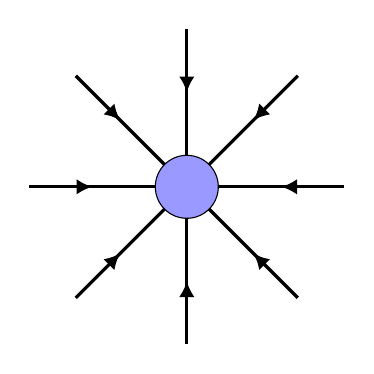
\begin{tikzpicture}
\begin{scope}[very thick,decoration={ markings, mark=at position 0.4 with {\arrow[]{Latex[length=2mm, width=2mm]}}}]
    \draw[postaction={decorate}] (0,2)--(0,0);
    \draw[postaction={decorate}] (0,-2)--(0,0);
    \draw[postaction={decorate}] (-2,0)--(0,0);
    \draw[postaction={decorate}] (2,0)--(0,0);
    \draw[postaction={decorate}] (1.41,1.41)--(0,0);
    \draw[postaction={decorate}] (1.41,-1.41)--(0,0);
    \draw[postaction={decorate}] (-1.41,1.41)--(0,0);
    \draw[postaction={decorate}] (-1.41,-1.41)--(0,0);
\end{scope}
\filldraw[fill=blue!40!white, draw=black] (0,0) circle (0.4cm);
\end{tikzpicture}
\caption{A radial graviatational field}
\end{figure}

If the same object is observed much more closely, radial field lines may appear parallel to one another and hence there is no change in the magnitude of \(g\) within the selected region of the gravitational field.

\begin{figure}[H]
\centering
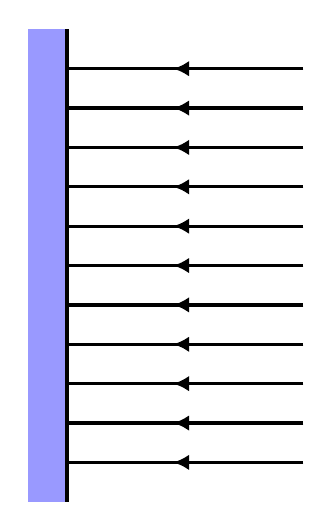
\begin{tikzpicture}
\fill[blue!40!white] (-2,3) rectangle (-1.5, -3);
\begin{scope}[very thick,decoration={ markings, mark=at position 0.55 with {\arrow[]{Latex[length=2mm, width=2mm]}}}]
    \draw[] (-1.5, 3) -- (-1.5, -3);
    \draw[postaction={decorate}]  (1.5,2.5) -- (-1.5,2.5);
    \draw[postaction={decorate}]  (1.5,2.0) -- (-1.5,2.0);
    \draw[postaction={decorate}]  (1.5,1.5) -- (-1.5,1.5);
    \draw[postaction={decorate}]  (1.5,1.0) -- (-1.5,1.0);
    \draw[postaction={decorate}]  (1.5,0.5) -- (-1.5,0.5);
    \draw[postaction={decorate}]  (1.5,0.0) -- (-1.5,0.0);
    \draw[postaction={decorate}]  (1.5,-0.5) -- (-1.5,-0.5);
    \draw[postaction={decorate}]  (1.5,-1.0) -- (-1.5,-1.0);
    \draw[postaction={decorate}]  (1.5,-1.5) -- (-1.5,-1.5);
    \draw[postaction={decorate}]  (1.5,-2.0) -- (-1.5,-2.0);
    \draw[postaction={decorate}]  (1.5,-2.5) -- (-1.5,-2.5);
\end{scope}
\end{tikzpicture}
\caption{A "uniform" graviatational field}
\end{figure}

\subsubsection{Gravitational Potential}
\label{sec:org4d0ee9d}

The \emph{gravitational potential} at a point in a gravitational field is the \emph{gravitational potential energy} per unit mass of a small test mass. It can also be described as the work done per unit mass to move an object from infinite distance to that point.

\begin{itemize}
\item The gravitational field around an object extends to \emph{infinity}. The strength of this field diminishes with distance from the centre of the object.

\item Any object within a gravitational field will have \emph{gravitational potential energy} (the energy of an object due to its position in a gravitational field).

\item For any object in a gravitational field, its \textbf{GPE} is least when it is close to the centre of the field and larger at greater distances from the centre of the field. \textbf{GPE} is \(0\) at the infinity position. Consequently, values of \textbf{GPE} closer to the centre of the field are negative.
\end{itemize}

The unit of gravitational potential is the \(Jkg^{-1}\) and like \textbf{GPE}, values are always negative. \textbf{GP} is expressed algebraically like this:

\[V = \dfrac{W}{M}\]

Points in a gravitational field which are the same distance from the centre of the field will share the same value of \(V\). These loci of points are called \emph{equipotentials} and no work is done against the gravitational field when an object moves along an equipotential.


\begin{figure}[H]
\centering
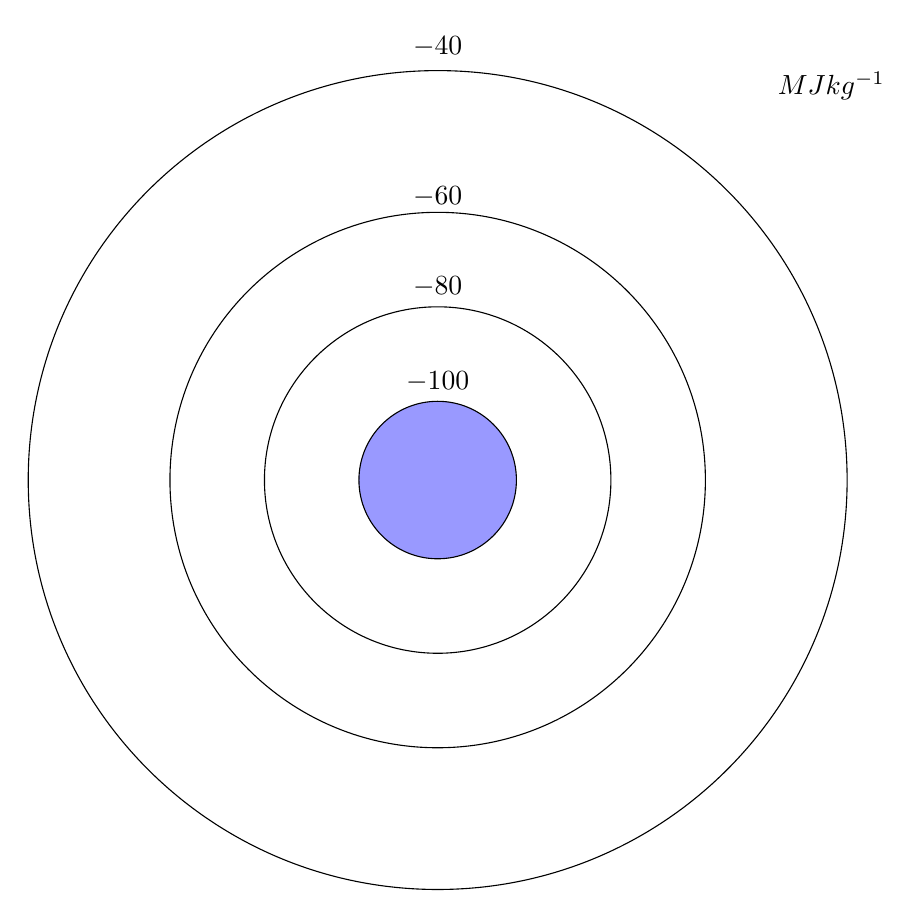
\begin{tikzpicture}
\begin{scope}[very thick,decoration={ markings, mark=at position 0.4 with {\arrow[]{Latex[length=2mm, width=2mm]}}}]
\end{scope}
\filldraw[fill=blue!40!white, draw=black] (0,0) circle (1cm);
\draw (0,0) circle (2.2cm);
\draw (0,0) circle (3.4cm);
\draw (0,0) circle (5.2cm);
\node[] at (0,1.25) {$-100$};
\node[] at (0,2.45) {$-80$};
\node[] at (0,3.6) {$-60$};
\node[] at (0,5.5) {$-40$};
\node[] at (5,5) {$MJkg^{-1}$};
\end{tikzpicture}
\caption{Equipotentials around a spherical body (not to scale)}
\end{figure}

\subsubsection{Potential Gradients}
\label{sec:orgc1bbf0c}

The \emph{potential gradient} at a point in a gravitational field is the change in potentail per metre at that point. As \(g\) decreases with distance from a given mass, the change in \(V\) per metre at greater distances from the centre of the field decreases. The potential gradient = \(\Delta V / \Delta r\), these values are labelled in the figure.

\begin{figure}[H]
\centering
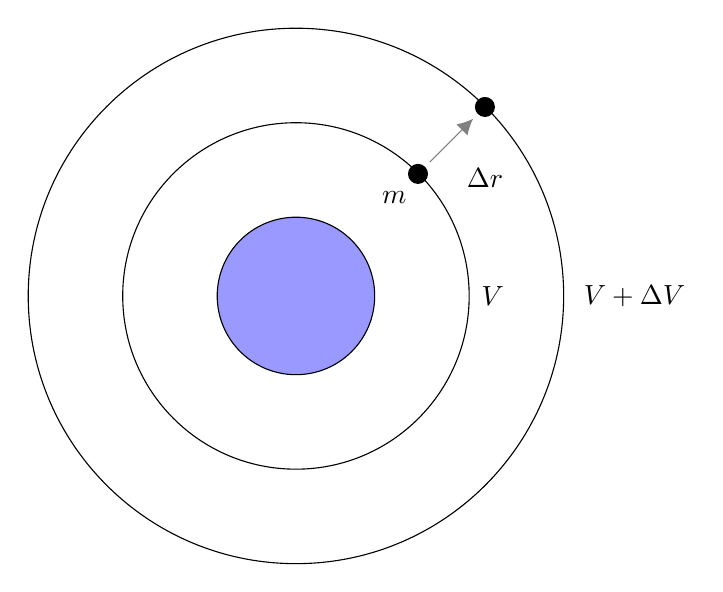
\begin{tikzpicture}
\begin{scope}[very thick,decoration={ markings, mark=at position 0.4 with {\arrow[]{Latex[length=2mm, width=2mm]}}}]
\end{scope}
\filldraw[fill=blue!40!white, draw=black] (0,0) circle (1cm);
\draw (0,0) circle (2.2cm);
\draw (0,0) circle (3.4cm);
\filldraw[black] (1.55, 1.55) circle (0.12cm);
\filldraw[black] (2.4, 2.4) circle (0.12cm);
\draw[-{Latex[length=2mm, width=2mm]}, gray] (1.7, 1.7) -- (2.25, 2.25);
\node[] at (1.25,1.25) {$m$};
\node[] at (2.5,0) {$V$};
\node[] at (4.3,0) {$V+ \Delta V$};
\node[] at (2.4,1.5) {$\Delta r$};
\end{tikzpicture}
\caption{Potential gradient}
\end{figure}

If the test mass \(m\) is moved a distance \(\Delta r\) away from the planet, its \textbf{GPE} will increase as it moves to a point of higher potential. A force must be applied to the object, which is equal and opposite to the force due to gravity, acting through \(\Delta r\).

\[\Delta W = F \Delta r\]

\[\Delta V = \dfrac{\Delta W}{m}\]

\[\Delta V = \dfrac{F \Delta r}{m}\]

\[F = \dfrac{m \Delta V}{\Delta r}\]

\[F_{grav} = -F\]

\[F_{grav} = - \dfrac{m \Delta V}{\Delta r}\]

\[g = \dfrac{F_{grav}}{m}\]

\[g = - \dfrac{\Delta V}{\Delta r}\]

This proves that the gravitational field strength is the negative of the potential gradient at any point, therefore it acts in the opposite direction (towards the planet).

\subsubsection{Law of Gravitation}
\label{sec:orgfa1844c}

Newton's law of gravitation describes an attractive force between any two point objects. It is directly proportional to the product of the masses of the two objects and inversely proportional to the square of the separation between the two points.

\[F = \dfrac{Gm_1m_2}{r^2}\]

The constant of proportionality \(G\) is called the \emph{universal constant of gravitation}. Its value is \(6.67 \times 10^{-11} \text{} Nm^2kg^{-2}\).

\subsubsection{Planetary Fields}
\label{sec:org74f4c1f}

The field of a large spherical body such as a planet is the same as if its mass were concentrated at a single central point. For a large point mass \(M\), the force exerted on a small test mass \(m\), where \(m < M\), at distance \(r\) is determined with Newton's law of gravitation.

\[F = \dfrac{GMm}{r^2}\]

The gravitational field strength \(g = F / m\) is equal to:

\[g = \dfrac{GM}{r^2}\]

These equations are true if \(r > R\), where \(R\) is the radius of the planetary body; At or beyond the radius of the planet, the value of \(M\) is constant and the proportionality is accurate. The surface gravitational field strength is a special form of the equation:

\[g_s = \dfrac{GM}{R^2}\]

\[GM = R^2g_s \]

\[g = \dfrac{GM}{r^2}\]

\[g = \dfrac{R^2g_s}{r^2}\]

Values of \(r\) that are smaller than \(R\) indicate positions within the planet itself. At these positions, only the mass located in the hypothetical sphere with radius of the original centre of the planet to the current position \(r\). Within the planet, \(g\) decreases along with \(r\) to 0 at the centre, as the mass at the exact centre is 0.

\[g = \dfrac{GM}{r^2}\]

\[V = \dfrac{4}{3} \pi r^3\]

\[M = \rho V = \dfrac{4}{3} \rho \pi r^3\]

\[g = \dfrac{G \dfrac{4}{3} \rho \pi r^3}{r^2}\]

\[g = \dfrac{4}{3} G \rho \pi r\]

This final form of the equation is true when \(r < R\).

\subsubsection{Satelite Motion}
\label{sec:org2b9ebb5}

\subsection{Electric Fields}
\label{sec:org6db6111}

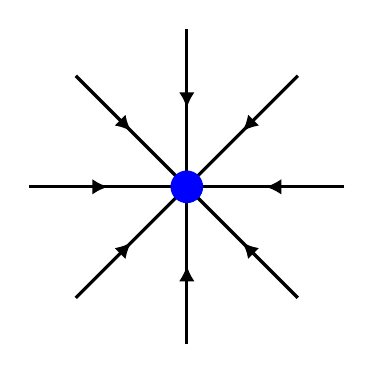
\begin{tikzpicture}
\begin{scope}[very thick,decoration={ markings, mark=at position 0.5 with {\arrow[]{Latex[length=2mm, width=2mm]}}}]
    \draw[postaction={decorate}] (0,2)--(0,0);
    \draw[postaction={decorate}] (0,-2)--(0,0);
    \draw[postaction={decorate}] (-2,0)--(0,0);
    \draw[postaction={decorate}] (2,0)--(0,0);
    \draw[postaction={decorate}] (1.41,1.41)--(0,0);
    \draw[postaction={decorate}] (1.41,-1.41)--(0,0);
    \draw[postaction={decorate}] (-1.41,1.41)--(0,0);
    \draw[postaction={decorate}] (-1.41,-1.41)--(0,0);
\end{scope}
\filldraw[blue] (0,0) circle (0.2cm);
\end{tikzpicture}

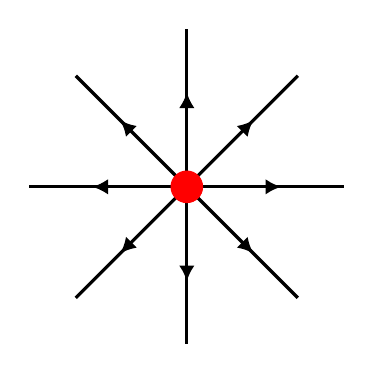
\begin{tikzpicture}
\begin{scope}[very thick,decoration={ markings, mark=at position 0.6 with {\arrow[]{Latex[length=2mm, width=2mm]}}}]
    \draw[postaction={decorate}] (0,0)--(0,2);
    \draw[postaction={decorate}] (0,0)--(0,-2);
    \draw[postaction={decorate}] (0,0)--(-2,0);
    \draw[postaction={decorate}] (0,0)--(2,0);
    \draw[postaction={decorate}] (0,0) -- (1.41,1.41);
    \draw[postaction={decorate}] (0,0) -- (1.41,-1.41);
    \draw[postaction={decorate}] (0,0) -- (-1.41,1.41);
    \draw[postaction={decorate}] (0,0) -- (-1.41,-1.41);
\end{scope}
\filldraw[red] (0,0) circle (0.2cm);
\end{tikzpicture}

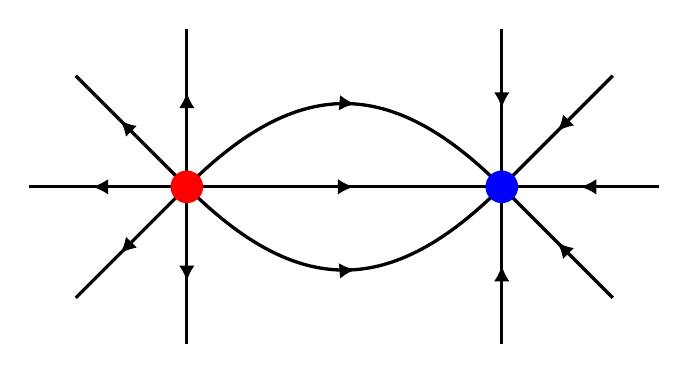
\begin{tikzpicture}
\filldraw[red] (-2, 0) circle (0.1cm);
\filldraw[blue] (2, 0) circle (0.1cm);
\begin{scope}[very thick,decoration={ markings, mark=at position 0.6 with {\arrow[]{Latex[length=2mm, width=2mm]}}}]
    \draw[postaction={decorate}] (-2,0)--(-4,0);
    \draw[postaction={decorate}] (-2,0)--(-2,2);
    \draw[postaction={decorate}] (-2,0)--(-2,-2);
    \draw[postaction={decorate}] (-2,0)--(-3.41,1.41);
    \draw[postaction={decorate}] (-2,0)--(-3.41,-1.41);
\end{scope}
\begin{scope}[very thick,decoration={ markings, mark=at position 0.5 with {\arrow[]{Latex[length=2mm, width=2mm]}}}]
    \draw[postaction={decorate}] (4,0) -- (2,0);
    \draw[postaction={decorate}] (2,2) -- (2,0);
    \draw[postaction={decorate}] (2,-2) -- (2,0);
    \draw[postaction={decorate}] (3.41,1.41) -- (2,0);
    \draw[postaction={decorate}] (3.41,-1.41) -- (2,0);
\end{scope}
\begin{scope}[very thick,decoration={ markings, mark=at position 0.53
with {\arrow[]{Latex[length=2mm, width=2mm]}}}]
    \draw[postaction={decorate}] (-2,0) -- (2,0);
    \draw[postaction={decorate}] (-2,0) .. controls (-0.59, 1.41) and (0.59, 1.41) .. (2,0);
    \draw[postaction={decorate}] (-2,0) .. controls (-0.59, -1.41) and (0.59, -1.41) .. (2,0);
\end{scope}
\filldraw[red] (-2, 0) circle (0.2cm);
\filldraw[blue] (2, 0) circle (0.2cm);
\end{tikzpicture}

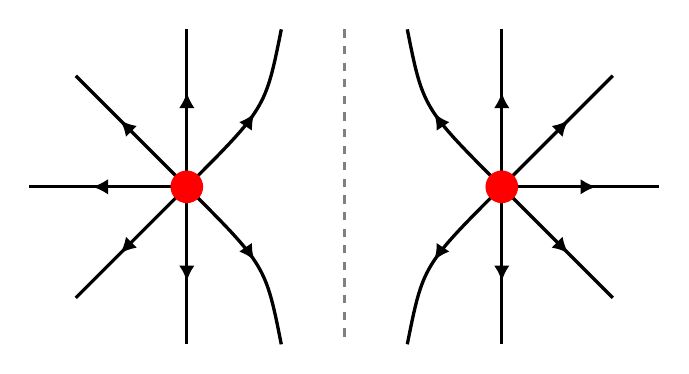
\begin{tikzpicture}
\begin{scope}[very thick,decoration={ markings, mark=at position 0.6 with {\arrow[]{Latex[length=2mm, width=2mm]}}}]
    \draw[postaction={decorate}] (-2,0)--(-4,0);
    \draw[postaction={decorate}] (-2,0)--(-2,2);
    \draw[postaction={decorate}] (-2,0)--(-2,-2);
    \draw[postaction={decorate}] (-2,0)--(-3.41,1.41);
    \draw[postaction={decorate}] (-2,0)--(-3.41,-1.41);
\end{scope}
\begin{scope}[very thick,decoration={ markings, mark=at position 0.6 with {\arrow[]{Latex[length=2mm, width=2mm]}}}]
    \draw[postaction={decorate}] (2,0)--(4,0);
    \draw[postaction={decorate}] (2,0)--(2,2);
    \draw[postaction={decorate}] (2,0)--(2,-2);
    \draw[postaction={decorate}] (2,0)--(3.41,1.41);
    \draw[postaction={decorate}] (2,0)--(3.41,-1.41);
\end{scope}
\begin{scope}[very thick,decoration={ markings, mark=at position 0.53
with {\arrow[]{Latex[length=2mm, width=2mm]}}}]
    \draw[postaction={decorate}] (-2,0) .. controls (-1, 1) .. (-0.8, 2);
    \draw[postaction={decorate}] (-2,0) .. controls (-1, -1) .. (-0.8, -2);
    \draw[postaction={decorate}] (2,0) .. controls (1, 1) .. (0.8, 2);
    \draw[postaction={decorate}] (2,0) .. controls (1, -1) .. (0.8, -2);
    \draw[gray, dashed] (0,2) -- (0, -2);
\end{scope}
\filldraw[red] (-2, 0) circle (0.2cm);
\filldraw[red] (2, 0) circle (0.2cm);
\end{tikzpicture}


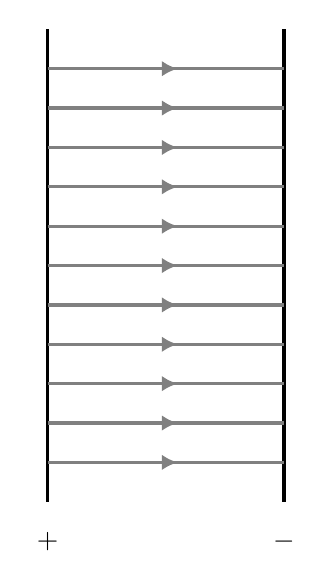
\begin{tikzpicture}
\begin{scope}[very thick,decoration={ markings, mark=at position 0.55 with {\arrow[]{Latex[length=2mm, width=2mm]}}}]
    \draw[] (-1.5, 3) -- (-1.5, -3);
    \draw[] (1.5, 3) -- (1.5, -3);
    \draw[postaction={decorate}, gray] (-1.5,2.5) -- (1.5,2.5);
    \draw[postaction={decorate}, gray] (-1.5,2.0) -- (1.5,2.0);
    \draw[postaction={decorate}, gray] (-1.5,1.5) -- (1.5,1.5);
    \draw[postaction={decorate}, gray] (-1.5,1.0) -- (1.5,1.0);
    \draw[postaction={decorate}, gray] (-1.5,0.5) -- (1.5,0.5);
    \draw[postaction={decorate}, gray] (-1.5,0.0) -- (1.5,0.0);
    \draw[postaction={decorate}, gray] (-1.5,-0.5) -- (1.5,-0.5);
    \draw[postaction={decorate}, gray] (-1.5,-1.0) -- (1.5,-1.0);
    \draw[postaction={decorate}, gray] (-1.5,-1.5) -- (1.5,-1.5);
    \draw[postaction={decorate}, gray] (-1.5,-2.0) -- (1.5,-2.0);
    \draw[postaction={decorate}, gray] (-1.5,-2.5) -- (1.5,-2.5);
\end{scope}
\node[] at (-1.5,-3.5) {$+$};
\node[] at (1.5,-3.5) {$-$};
\end{tikzpicture}

\section{Nuclear Physics}
\label{sec:org2765f0b}
\subsection{Radiation}
\label{sec:orgf92ffae}

Three types of radiation:

\begin{enumerate}
\item Alpha: \(^4_2\alpha\)
\item Beta: \(^{ \text{ } \text{ }0}_{-1}\beta^-\) / \(^{0}_{1}\beta^+\)
\item Gamma: \(\gamma\)
\end{enumerate}

\subsubsection{Alpha Emission}
\label{sec:org3459f5a}

An \(\alpha\) particle is composed of two neutrons and two protons. \(\alpha\) emission results in a different, smaller nuclide.

\[^A_ZX \rightarrow \text{} ^4_2\alpha + \text{} ^{A-4}_{Z-2}Y\]

\subsubsection{Beta Minus Decay}
\label{sec:orga7f4a4c}

A \(\beta^-\) particle is an electron. During \(\beta^-\) emission, a neutron in a neutron-rich nucleus decays into a proton. The underlying change is the conversion of a \emph{down quark} into an \emph{up quark}.

\[^A_ZX \rightarrow \text{} ^{ \text{ } \text{ }0}_{-1}\beta + \text{} ^{\text{ } \text{ }A}_{Z+1}Y + \bar{\nu}_e\]


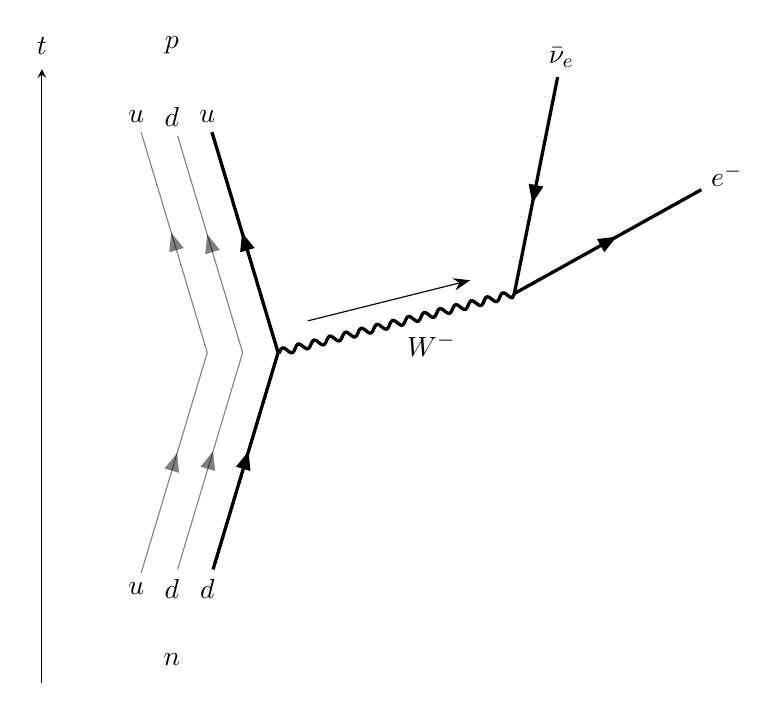
\begin{tikzpicture}[x=30mm, y=30mm]
\begin{feynman}
    \vertex (i1) {\(u\)};
    \vertex[right=.15 of i1] (i2) {\(d\)};
    \vertex[right=.15 of i2] (i3) {\(d\)};
    \vertex[below=.3 of i2] (n) {\(n\)};

    \vertex[above=2 of i1] (f1) {\(u\)};
    \vertex[right=.15 of f1] (f2) {\(d\)};
    \vertex[right=.15 of f2] (f3) {\(u\)};
    \vertex[above=.3 of f2] (p) {\(p\)};

    \vertex[above=1 of i3] (a);
    \vertex[right=.15 of a] (b);
    \vertex[right=.15 of b] (c);

    \vertex at ($(c) + (1,.25)$) (d);
    \vertex at ($(d) + (.2, 1)$) (f4) {\(\bar{\nu}_e\)};
    \vertex at ($(d) + (.9,.5)$) (f5) {\(e^-\)};
\diagram*{
    (i1) -- [fermion, opacity=0.5] (a) -- [fermion, opacity=0.5] (f1),
    (i2) -- [fermion, opacity=0.5] (b) -- [fermion, opacity=0.5] (f2),
    (i3) -- [fermion, very thick] (c) -- [fermion, very thick] (f3),
    (c) -- [boson, edge label'=\(W^-\), momentum, very thick] (d),
    (d) -- [fermion, very thick] (f5),
    (d) -- [anti fermion, very thick] (f4),
};

\draw[-stealth] (-.4,-.4) -- (-.4,2.2);
\node at (-.4,2.3) {\(t\)};
\end{feynman}
\end{tikzpicture}

\subsubsection{Beta Plus Decay}
\label{sec:org7710ab6}

A \(\beta^+\) particle is a positron. During \(\beta^+\) emission, a proton in a proton-rich nucleus decays into a neutron. The underlying change is the conversion of an \emph{up quark} into an \emph{down quark}.

\[^A_ZX \rightarrow \text{} ^{ \text{ } \text{ }0}_{+1}\beta + \text{} ^{\text{ } \text{ }A}_{Z-1}Y + \nu_e\]


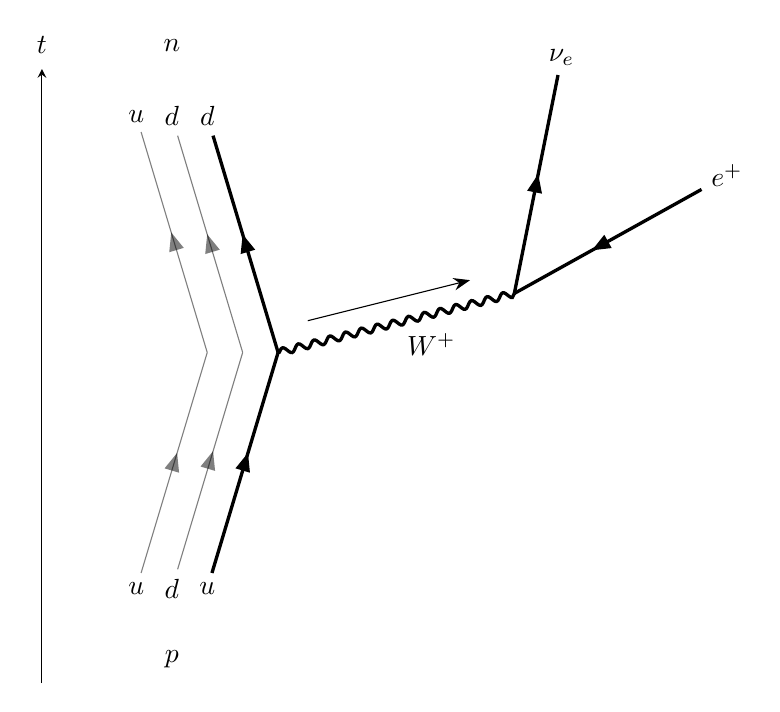
\begin{tikzpicture}[x=30mm, y=30mm]
\begin{feynman}
    \vertex (i1) {\(u\)};
    \vertex[right=.15 of i1] (i2) {\(d\)};
    \vertex[right=.15 of i2] (i3) {\(u\)};
    \vertex[below=.3 of i2] (n) {\(p\)};

    \vertex[above=2 of i1] (f1) {\(u\)};
    \vertex[right=.15 of f1] (f2) {\(d\)};
    \vertex[right=.15 of f2] (f3) {\(d\)};
    \vertex[above=.3 of f2] (p) {\(n\)};

    \vertex[above=1 of i3] (a);
    \vertex[right=.15 of a] (b);
    \vertex[right=.15 of b] (c);

    \vertex at ($(c) + (1,.25)$) (d);
    \vertex at ($(d) + (.2, 1)$) (f4) {\(\nu_e\)};
    \vertex at ($(d) + (.9,.5)$) (f5) {\(e^+\)};
\diagram*{
    (i1) -- [fermion, opacity=0.5] (a) -- [fermion, opacity=0.5] (f1),
    (i2) -- [fermion, opacity=0.5] (b) -- [fermion, opacity=0.5] (f2),
    (i3) -- [fermion, very thick] (c) -- [fermion, very thick] (f3),
    (c) -- [boson, edge label'=\(W^+\), momentum, very thick] (d),
    (d) -- [anti fermion, very thick] (f5),
    (d) -- [fermion, very thick] (f4),
};

\draw[-stealth] (-.4,-.4) -- (-.4,2.2);
\node at (-.4,2.3) {\(t\)};
\end{feynman}
\end{tikzpicture}

\subsubsection{Electron Capture}
\label{sec:org2a67f59}

A proton-rich nucleus could also undergo \emph{electron capture}. In this type of decay a proton changes into a neutron after capturing an inner shell electron.

\[^A_ZX + ^{ \text{ } \text{ }0}_{-1}\beta \rightarrow \text{} ^{\text{ } \text{ }A}_{Z-1}Y + \nu_e\]


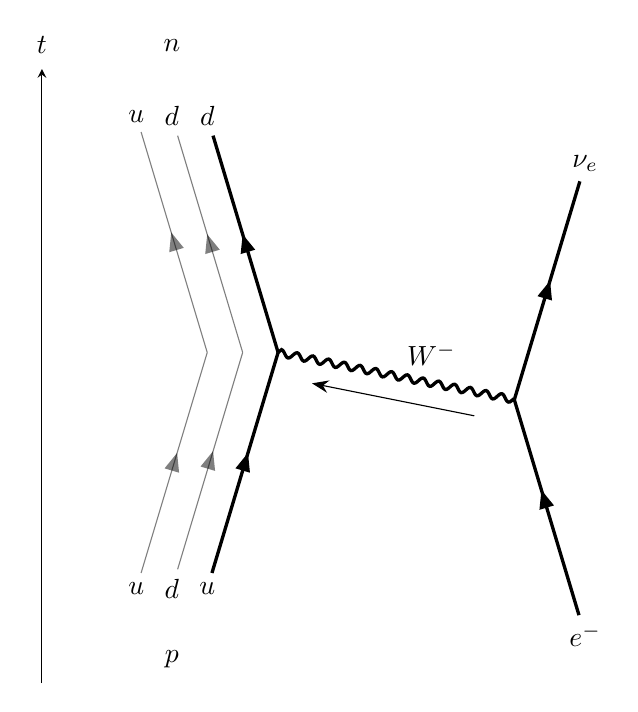
\begin{tikzpicture}[x=30mm, y=30mm]
\begin{feynman}
    \vertex (i1) {\(u\)};
    \vertex[right=.15 of i1] (i2) {\(d\)};
    \vertex[right=.15 of i2] (i3) {\(u\)};
    \vertex[below=.3 of i2] (n) {\(p\)};

    \vertex[above=2 of i1] (f1) {\(u\)};
    \vertex[right=.15 of f1] (f2) {\(d\)};
    \vertex[right=.15 of f2] (f3) {\(d\)};
    \vertex[above=.3 of f2] (p) {\(n\)};

    \vertex[above=1 of i3] (a);
    \vertex[right=.15 of a] (b);
    \vertex[right=.15 of b] (c);

    \vertex at ($(c) + (1,-.2)$) (d);
    \vertex at ($(d) + (.3, 1)$) (f4) {\(\nu_e\)};
    \vertex at ($(d) + (.3,-1)$) (f5) {\(e^-\)};
\diagram*{
    (i1) -- [fermion, opacity=0.5] (a) -- [fermion, opacity=0.5] (f1),
    (i2) -- [fermion, opacity=0.5] (b) -- [fermion, opacity=0.5] (f2),
    (i3) -- [fermion, very thick] (c) -- [fermion, very thick] (f3),
    (d) -- [boson, edge label'=\(W^-\), momentum, very thick] (c),
    (d) -- [anti fermion, very thick] (f5),
    (d) -- [fermion, very thick] (f4),
};

\draw[-stealth] (-.4,-.4) -- (-.4,2.2);
\node at (-.4,2.3) {\(t\)};
\end{feynman}
\end{tikzpicture}

The nature of the \emph{W boson} is not significant/distinguishable. The same diagram could be written:


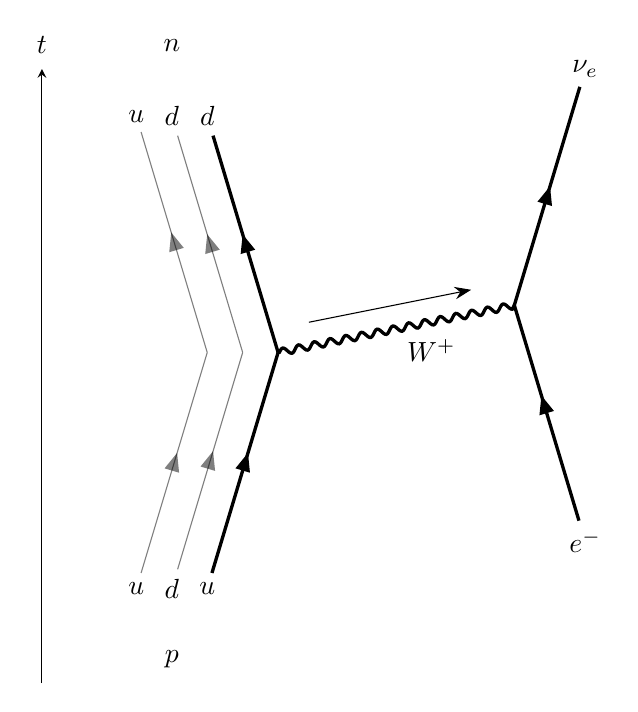
\begin{tikzpicture}[x=30mm, y=30mm]
\begin{feynman}
    \vertex (i1) {\(u\)};
    \vertex[right=.15 of i1] (i2) {\(d\)};
    \vertex[right=.15 of i2] (i3) {\(u\)};
    \vertex[below=.3 of i2] (n) {\(p\)};

    \vertex[above=2 of i1] (f1) {\(u\)};
    \vertex[right=.15 of f1] (f2) {\(d\)};
    \vertex[right=.15 of f2] (f3) {\(d\)};
    \vertex[above=.3 of f2] (p) {\(n\)};

    \vertex[above=1 of i3] (a);
    \vertex[right=.15 of a] (b);
    \vertex[right=.15 of b] (c);

    \vertex at ($(c) + (1,.2)$) (d);
    \vertex at ($(d) + (.3, 1)$) (f4) {\(\nu_e\)};
    \vertex at ($(d) + (.3,-1)$) (f5) {\(e^-\)};
\diagram*{
    (i1) -- [fermion, opacity=0.5] (a) -- [fermion, opacity=0.5] (f1),
    (i2) -- [fermion, opacity=0.5] (b) -- [fermion, opacity=0.5] (f2),
    (i3) -- [fermion, very thick] (c) -- [fermion, very thick] (f3),
    (c) -- [boson, edge label'=\(W^+\), momentum, very thick] (d),
    (d) -- [anti fermion, very thick] (f5),
    (d) -- [fermion, very thick] (f4),
};

\draw[-stealth] (-.4,-.4) -- (-.4,2.2);
\node at (-.4,2.3) {\(t\)};
\end{feynman}
\end{tikzpicture}

\subsubsection{Gamma Emission}
\label{sec:org1a68bc4}

There is no change to the number of nucleons in the nucleus when a \(\gamma\) photon is emitted. This type of emission usually happens if the nucleus is in an excited state after one of the previous types of emission.

\subsection{Inverse Square Law}
\label{sec:orgc3bca71}

The intensity \(I\) of \(\gamma\) radiation is the energy transferred per second per unit area. Assuming a point source emits \(n\) \(\gamma\) photons per second and each photon has the energy \(hf\), the total energy emitted by the source per second is \(nhf\). These photons are free to leave the source in any direction, so at distance \(r\) from the source all the photons will pass through an area equal to the \emph{S.A.} of a sphere with radius \(r\). This equation represents the intensity of radiation from a point source at distance \(r\):

\[I = \dfrac{nhf}{4 \pi r^2}\]

\subsection{Hazards of Radiation}
\label{sec:org52b34ae}

Ionising radiation is damaging to living cells. It may cause cells to die, mutate or grow uncontrollably. The consequences may be felt by the affected individual, which is described as \emph{somatic effects}, or passed onto future generations \emph{genetically}.

To best mitigate the risks of radiation, sources should be kept in \emph{lead-lined} containers to reduce any \(\gamma\) emission from the source to background level. These sources may be kept in a secure, locked-away location and exposure / use of the source should be recorded.

During use, solid sources should be handled with handling tools, to keep the source at a distance from the body. This reduces the intensity of \(\gamma\) radiation incident on the handler and would ideally put their body beyond the range of \(\alpha\) or \(\beta\) particles. Liquid, gaseous and powdered sources should be kept in sealed containers, so they are not accidentally inhaled, ingested or split.

\subsection{Radioactive Decay}
\label{sec:org40e1c19}

If a radioactive isotope of element \(X\) undergoes \(\alpha\) or \(\beta\) emission, it is no longer a nucleus of the same element, due to the change in proton number. If this nucleus was one of many in a sample of a particular isotope, the number of nuclei of this isotope will decrease as individual nuclei decay. The same relationship is true of the mass of the original isotope; the mass will decrease as nuclei decay. There are three important quantities surrounding radioactive decay:

\begin{itemize}
\item The \emph{half-life} \(T_{1/2}\) of a radioactive isotope is the time take for the mass (or any other specific property) to decrease to half the initial value.

\item The \emph{activity} \(A\) of a radioactive isotope is the number of nuclei disintegrating per second, corresponds to the rate of changes of nuclei of the initial isotope. The unit of activity is the \emph{Becquerel} (Bq), where 1Bq is one disintegration per second.

\item The \emph{decay constant} \(\lambda\) is the probability of an individual nucleus decaying per unit time (usually one second).
\end{itemize}

The decay of a single nucleus is impossible to predict. Every nucleus of an isotope in a sample has an equal probability of decaying in a given interval. For a large sample of a radioactive isotope \(X\), the number of nuclei which disintegrate \(\Delta N\) in a given time period \(\Delta t\) is related to the initial number of nuclei \(N_0\), via the decay constant.

\subsubsection{Decay Constant}
\label{sec:orgce35a3f}

The probability of a single decay is the fraction of the initial number of nuclei of \(X\) which decay per second. This is called the \emph{decay constant}, and is represented with the symbol \(\lambda\). If reference is made to \emph{decay} or its decreasing nature, there is no need to include a minus sign.

\[\lambda = \dfrac{\Delta N}{N_0}/\Delta t\]

The change in number of nuclei for a combination of the given factors can be obtained by rearranging the equation above. Note the presence of the minus sign here indicating decrease.

\[ \Delta N = - \lambda N_0 \Delta t\]

\subsubsection{Activity}
\label{sec:org11b74d0}

The activity of the isotope is the number of nuclei which disintegrate per second and it is proportional to the value of \(N_0\). An expression for \(A\) can be obtained as follows:

\[ \dfrac{\Delta N}{\Delta t} = - \lambda N_0\]

\[ A = - \lambda N_0\]

Therefore the activity of \(N\) nuclei of a particular isotope can also be written simply:

\[ A = \lambda N\]

\subsubsection{Decay Curves}
\label{sec:org498ccb0}

As the activity, or rate of change of nuclei of \(X\), is proportional to the current number of nuclei \(N\) of \(X\), the relationship between \(t\) and \(N\) is one of exponential decay. The number of nuclei remaining after a particular time period is proportional to \(N_0\).

\[N = N_0 e^{- \lambda t}\]

\begin{center}
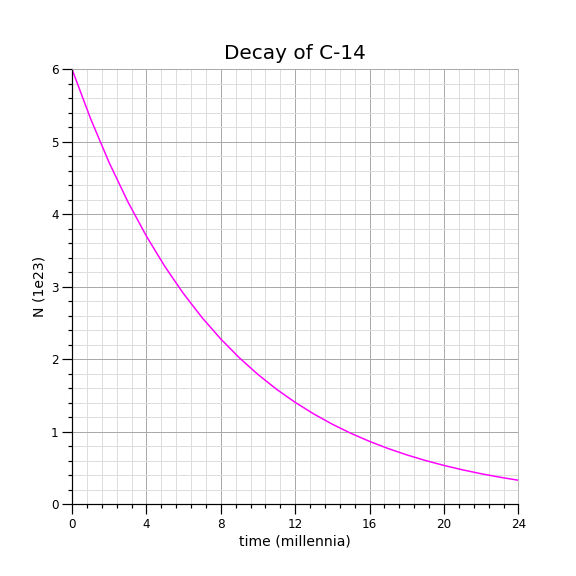
\includegraphics[width=.9\linewidth]{./images/c-14_decay.png}
\end{center}

Both activity and mass are directly related to the number of nuclei.

\[m = m_0 e^{- \lambda t}\]
\[A = A_0 e^{- \lambda t}\]

\subsubsection{Half-life}
\label{sec:org103ff67}

Half-life can be linked to the decay constant. When \(t= T_{1/2}\), the number of nuclei remaining is \(N = 0.5N_0\). With these equations, substitutions can be made:

\(0.5N_0 = N_0 e^{-\lambda T_{1/2}}\)

\(0.5 = e^{-\lambda T_{1/2}}\)

\(\ln (0.5) = -\lambda T_{1/2}\)

\(-\ln (0.5) = \lambda T_{1/2}\)

\(\ln (0.5^{-1}) = \lambda T_{1/2}\)

\(\ln (2) = \lambda T_{1/2}\)

\(T_{1/2} = \dfrac{\ln(2)}{\lambda}\)

\begin{center}
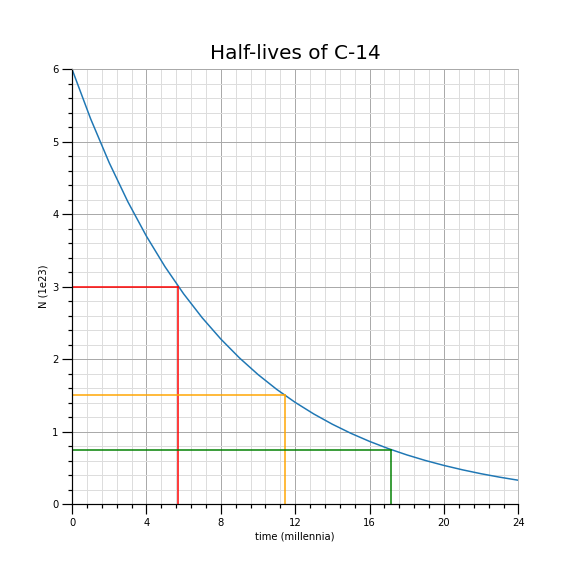
\includegraphics[width=.9\linewidth]{./images/c-14_t_half.png}
\end{center}

\subsection{Nuclear Radius}
\label{sec:org8f3dedb}

The radius of a nucleus is proportional to the cube root of the nucleon number and the constant \(r_0\), which is equal to 1.05fm.

\[R = r_0 A^{1/3}\]

\[V = \dfrac{4}{3} \pi R^3 = \dfrac{4}{3} \pi (r_0 A^{1/3})^3 = \dfrac{4}{3} \pi {r_0}^3 A\]

Seeing as the mass of a nucleus is equal to \(Au\), where \(u\) is the atomic mass unit, the density of any nucleus is constant.

\(\rho = \dfrac{Au}{4/3 \text{ } \pi {r_0}^3 A} = \dfrac{1u}{4/3 \text{ } \pi {r_0}^3}\)

When evaluated, the density of a nucleus of any element is \(3.4 \times 10^{17}\).

\subsection{Energy and Mass}
\label{sec:orgc71be94}

The equation \(E = mc^2\) links the energy of an object to the change of its mass and the speed of light in free space. Consequently, the mass of any object changes as it gains or loses energy. This is only significant on the nuclear/sub-nuclear scale. The energy released during a reaction is \(Q = \Delta mc^2\), where \(\Delta m\) is the difference in mass before and after the interaction.

\subsection{Binding Energy}
\label{sec:orgce0b40a}

The binding energy of a nucleus is the work done to separate all of the protons and neutrons from the nucleus. When a nucleus is formed from individual nucleons, energy is released amounting to the binding energy of the nucleus. Due to this release of energy the mass of the nucleus is less than the sum of the masses of constituent nucleons.

The mass defect \(\Delta m\) of a nucleus is the difference between the sum of the masses of separated nucleons and the mass of the whole nucleus. The mass defect for a \(^A_ZX\) nucleus can be calculated with this equation.

\[\Delta m =  Zm_p + (A-Z)m_n - M_{\text{NUC}} \]

Where \(m_p\) and \(m_n\) are the masses of a proton and a neutron respectively and \(M_{\text{NUC}}\) is the mass of the whole nucleus. The binding energy is equal to: \(Q = \Delta mc^2\). The values of \(m_p\) and \(m_n\) are often quoted in terms of \(u\), the atomic mass unit.

\begin{itemize}
\item \(1u = 1.661 \times 10^{-27}kg= 931.3MeV\)
\item \(m_p = 1.00728u\)
\item \(m_n = 1.00867u\)
\end{itemize}

\subsection{Quantum Tunnelling}
\label{sec:orgeee974b}

Two protons and two neutrons in a nucleus may bind together to as a cluster, which may be ejected from the nucleus as an \(\alpha\) particle. The \(\alpha\) particle is given a large amount of energy during its formation.

\subsection{Nuclear Stability}
\label{sec:orgd3fdb92}

Each nucleus has a binding energy and a specific binding energy per nucleon. This is the binding energy divided by the nucleon number of the nucleus. This value is indicative of the stability of the nucleus. More stable nuclei have a larger binding energy per nucleon. The maximum value is approximately 8.7Mev, occurring in the region \(50 \le A \le 60\).

\begin{center}
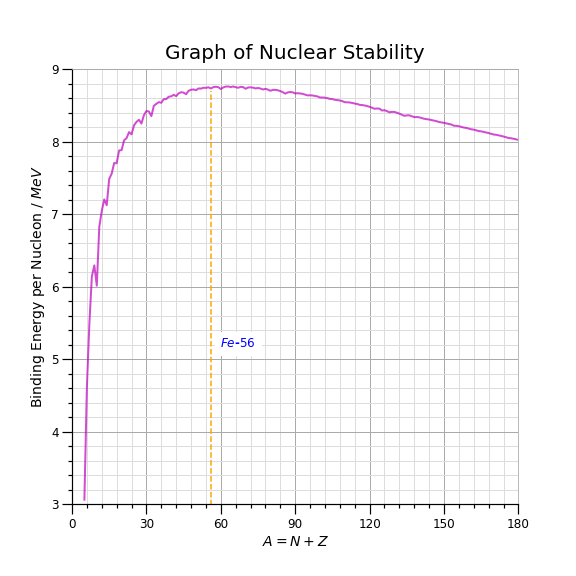
\includegraphics[width=.9\linewidth]{./images/nuclear_stability.png}
\end{center}

The orange line in the figure indicates the position of Fe-56, a very stable isotope of Iron. Energy is released in nuclear events under certain conditions:

\begin{itemize}
\item Fusion of nuclei to the left of the division. When heavier nuclei are formed energy is released due to the greater binding energy per nucleon of the resulting nuclei.

\item Fission of nuclei to the right of the division. When multiple, lighter daughter nuclei are formed energy is released due to the greater binding energy per nucleon of the resulting nuclei.
\end{itemize}
\end{document}
